\let\lesson\undefined
\newcommand{\lesson}{\phantomlesson{Bài 18: Động lượng.}}
\chapter[Động lượng]{Động lượng}
\setcounter{section}{0}
\section{Lý thuyết}
\subsection{Động lượng của một vật}
\begin{minipage}{0.6\textwidth}
	Động lượng $\vec{p}$ của một vật khối lượng $m$ đang chuyển động với vận tốc $\vec{v}$ là đại lượng được xác định bởi công thức:
	\begin{equation*}
		\vec{p}=m\vec{v}
	\end{equation*}
	trong đó:
	\begin{itemize}
		\item $\vec{p}$: động lượng của vật, đơn vị trong hệ SI là $\si{\kilogram\cdot\meter/\second}$;
		\item $m$: khối lượng của vật, đơn vị trong hệ SI là $\si{\kilogram}$;
		\item $\vec{v}$: vận tốc của vật, đơn vị trong hệ SI là $\si{\meter/\second}$.
	\end{itemize}
	Động lượng là một đại lượng vector cùng hướng với vận tốc của vật.
\end{minipage}
\begin{minipage}{0.4\textwidth}
	\begin{center}
		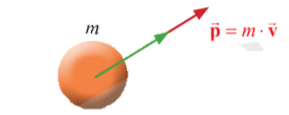
\includegraphics[scale=0.7]{../figs/G10-023-1}
	\end{center}
\end{minipage}
\subsection{Tổng động lượng của hệ vật}
%\vspace{-0.5cm}
\subsubsection{Động lượng hệ nhiều vật}

Động lượng của hệ là tổng động lượng của các vật trong hệ

\begin{equation*}
	\vec {p} = \vec {p_1} + \vec{p_2}+\vec{p_3}+...
\end{equation*}
\subsubsection{Các trường hợp đặc biệt}
\begin{itemize}
	\item \textbf{Trường hợp 1: Hai vector động lượng cùng phương cùng chiều} 
	\begin{center}
		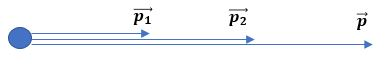
\includegraphics[scale=0.6]{../figs/VN10-PH-29-L-021-2-1.JPG}
	\end{center}
	\begin{equation*}
		\vec {p} = \vec {p_1} + \vec{p_2}.
	\end{equation*}
	
	vector động lượng của hệ $\vec{p}$ có 
	\begin{itemize}
		\item Phương và chiều: cùng phương cùng chiều với vector động lượng của mỗi vật.
		\item Độ lớn: $$p=p_1+p_2.$$ 
	\end{itemize}
	
	\item \textbf{Trường hợp 2: Hai vector động lượng cùng phương ngược chiều}
	\begin{center}
		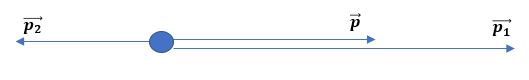
\includegraphics[scale=0.6]{../figs/VN10-PH-29-L-021-2-2.JPG}
	\end{center}
	\begin{equation*}
		\vec {p} = \vec {p_1} + \vec{p_2}.
	\end{equation*}
	vector động lượng của hệ $\vec{p}$ có 
	\begin{itemize}
		\item Phương và chiều: cùng phương cùng chiều với vector động lượng của vật có giá trị lớn hơn.
		\item Độ lớn: $$p=|p_1-p_2|.$$
	\end{itemize}
	
	\item \textbf{Trường hợp 3: Hai vector động lượng vuông góc}
	\begin{center}
		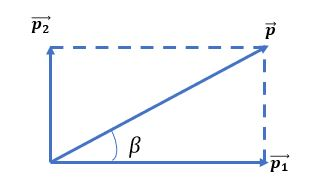
\includegraphics[scale=0.6]{../figs/VN10-PH-29-L-021-2-3.JPG}
	\end{center}
	\begin{equation*}
		\vec {p} = \vec {p_1} + \vec{p_2}.
	\end{equation*}
	vector động lượng của hệ $\vec{p}$ có 
	\begin{itemize}
		\item Phương và chiều: là đường chéo của hình chữ nhật xác định bởi góc $\beta$ với $\tan \beta = {p_2}/{p_1}.$
		\item Độ lớn: $$p = \sqrt {p_1^2+p^2_2}.$$
	\end{itemize}
	
	\item \textbf{Trường hợp 4: Hai vector động lượng tạo với nhau một góc $\alpha$}
	\begin{center}
		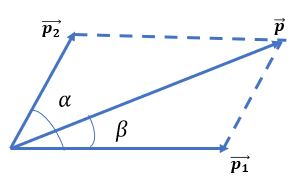
\includegraphics[scale=0.6]{../figs/VN10-PH-29-L-021-2-4.JPG}
	\end{center}
	\begin{equation*}
		\vec {p} = \vec {p_1} + \vec{p_2}.
	\end{equation*}
	vector động lượng của hệ $\vec{p}$ có 
	\begin{itemize}
		\item Phương và chiều: là đường chéo của hình bình hành xác định bởi góc $\beta$ tính bởi 
		\begin{equation*}
			\cos \beta = \dfrac  {p_1^2+p^2-p_2^2}{2p_1p} \qquad\text{hoặc}\qquad
			\tan\beta = \dfrac{p_2\sin\alpha}{p_1+p_2\cos\alpha}
		\end{equation*}
		\item Độ lớn  $$p = \sqrt{p^2_1+p^2_2 - 2p_1p_2 \cos (180^\circ - \alpha)} = \sqrt{p^2_1+p^2_2 + 2p_1p_2 \cos  \alpha}.$$
	\end{itemize}
	
	\textit{Lưu ý:} Nếu hệ gồm nhiều hơn 2 vật, ta có thể đưa bài toán tìm động lượng của hệ nhiều vật thành bài toán tìm động lượng của hệ 2 vật, bằng cách nhóm lần lượt hai động lượng và tiến hành cộng như hệ 2 vật.	Ví dụ ta xét hệ 3 vật, ta có thể cộng động lượng hai vật đầu tiên rồi cộng tiếp với động lượng vật thứ ba:
	\begin{equation*}
		\vec{p}=\vec{p_1}+ \vec{p_2}+ \vec{p_3} = (\vec{p_1}+ \vec{p_2}) + \vec{p_3} = \vec{p_{12}} + \vec{p_3}.
	\end{equation*}
	
	
	
\end{itemize}
\subsection{Xung lượng. Độ biến thiên động lượng}
\subsubsection{Xung lượng của lực}
\begin{itemize}
	\item Khi một lực $\vec{F}$ không đổi tác dụng lên một vật trong khoảng thời gian $\Delta t$ thì tích $\vec{F} \Delta t$ được định nghĩa là xung lượng của lực $\vec{F}$ trong khoảng thời gian $\Delta t$ ấy. 
	\item Trong hệ SI, đơn vị xung lượng của lực là $N \cdot s$.
\end{itemize}
\subsubsection{Mối liên hệ giữa độ biến thiên động lượng và xung lượng của lực}
Độ biến thiên động lượng của một vật trong khoảng thời gian $\Delta t$ bằng xung lượng của tổng các lực tác dụng lên vật trong khoảng thời gian đó.
\begin{equation*}
	\Delta \vec{p}=\vec{p_2} - \vec{p_1} =\vec{F} \Delta t \qquad\text{hay}\qquad \vec{F}=\dfrac{\Delta\vec{p}}{\Delta t}
\end{equation*}
\luuy{Công thức $\vec{F}=\dfrac{\Delta\vec{p}}{\Delta t}$ được xem là một cách diễn đạt khác của định luật II Newton:
	\begin{center}
		\emph{Lực tác dụng lên vật bằng tốc độ thay đổi động lượng của vật.}
	\end{center}
}
\section{Mục tiêu bài học - Ví dụ minh họa}
\begin{dang}{Xác định động lượng của một vật}
	\viduii{2}{Một ô tô có khối lượng $\SI{1000}{kg}$, chạy với vận tốc $\SI{54}{km/h}$. Tính động lượng của ô tô.
	}
	{\hide{Đổi $v=\SI{54}{km/h} = \SI{15}{m/s}$.
			
			Động lượng của ô tô:
			$p = mv =\SI{1000}{kg} \cdot \SI{15}{m/s}= \SI{15000}{kg.m/s}$.}
	}
		\viduii{2}{Một vật có khối lượng $\SI{2}{\kilogram}$ và có động lượng $\SI{6}{\kilogram\cdot\meter/\second}$. Vật đang chuyển động với tốc độ bao nhiêu?
	}
	{\hide{Tốc độ của vật: $$v=\dfrac{p}{m}=\dfrac{\SI{6}{kg.m/s}}{\SI{2}{\kilogram}}=\SI{3}{m/s}.$$}
	}
	\viduii{3}{Tại thời điểm $t_0=0$, một vật có khối lượng $m = 500\ \text{g}$ rơi tự do không vận tốc đầu từ độ cao 80 m xuống đất với $g=\SI{10}{\meter/\second^2}$. Động lượng của vật tại thời điểm $t = 2\ \text{s}$ có
		
		\begin{mcq}
			\item độ lớn 10 kg $\cdot$ m/s; phương thẳng đứng chiều từ dưới lên trên.
			\item độ lớn 10000 kg $\cdot$ m/s; phương thẳng đứng chiều từ trên xuống dưới.
			\item độ lớn 10 kg $\cdot$ m/s; phương thẳng đứng chiều từ trên xuống dưới.
			\item độ lớn 10000 kg $\cdot$ m/s; phương thẳng đứng chiều từ dưới lên trên.
		\end{mcq}
	}
	{		\hide{\begin{center}
				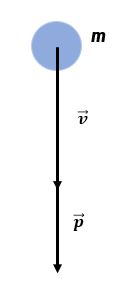
\includegraphics[scale=0.6]{../figs/VN10-PH-29-L-021-1-1.JPG}
			\end{center}
			\begin{itemize}
				\item Vecto vận tốc của vật trong chuyển động rơi tự do sau 2 giây có độ lớn 
				\begin{equation*}
					v=g  t =\SI{10}{\meter/\second^2}\cdot\SI{2}{\second}= 20 \ \text{m/s}.
				\end{equation*}
				và có chiều hướng thẳng xuống dưới.
				
				\item Động lượng của vật sau 2 giây là vector có độ lớn 			
				\begin{equation*}
					p=mv= \SI{0.5}{\kilogram}\cdot\SI{20}{\meter/\second}=10\ \text{kg} \cdot \text{m/s}.
				\end{equation*}
				và có chiều từ trên xuống dưới như hình vẽ.
			\end{itemize}
			
			\textbf{Đáp án: C}.}
	}
\end{dang}

\begin{dang}{Xác định tổng động lượng của hệ vật}
	\viduii{2}{Hệ gồm hai vật có khối lượng lần lượt là $m_1=\SI{3}{kg}$, $m_2=\SI{6}{kg}$, chuyển động với vận tốc có độ lớn lần lượt là $v_1=\SI{2}{m/s}$, $v_2=\SI{1}{m/s}$. Tính độ lớn tổng động lượng của hệ trong trường hợp
		\begin{enumerate}[label=\alph*)]
			\item hai vật chuyển động cùng phương ngược chiều.
			\item hai vật chuyển động cùng phương cùng chiều.
		\end{enumerate}
	}
	{\hide{Động lượng của hệ: $\vec p = \vec p_1 + \vec p_2$.
			\begin{enumerate}[label=\alph*)]
				\item Vì hai vật chuyển động cùng phương ngược chiều nên $p=|p_1-p_2| = |m_1v_1 - m_2v_2| = 0$.
				\item Vì hai vật chuyển động cùng phương cùng chiều nên $p=p_1+p_2=m_1v_1+ m_2v_2 =\SI{12}{\kilogram\cdot\meter/\second}$.
		\end{enumerate}}
	}
	\viduii{2}{Hai vật 1 và 2 chuyển động thẳng đều trên cùng một đường thẳng AB, cùng chiều từ A đến B có khối lượng và tốc độ tương ứng với mỗi vật là $m_1=\SI{5}{\kilogram}$, $v_1=\SI{36}{\kilo\meter/\hour}$, $m_2=\SI{4}{\kilogram}$, $v_2=\SI{15}{\meter/\second}$. vector tổng động lượng của hệ hai xe có
		\begin{mcq}
			\item độ lớn $240\ \text{kg} \cdot \text{m/s}$; phương là đường thẳng AB chiều từ A đến B.
			\item độ lớn $110\ \text{kg} \cdot \text{m/s}$; phương là đường thẳng AB chiều từ A đến B. 
			\item độ lớn $240\ \text{kg} \cdot \text{m/s}$; phương là đường thẳng AB chiều từ B đến A.
			\item độ lớn $110\ \text{kg} \cdot \text{m/s}$; phương là đường thẳng AB chiều từ B đến A.
		\end{mcq}
	}
	{	\hide{	\begin{center}
				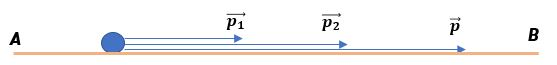
\includegraphics[scale=0.6]{../figs/VN10-PH-29-L-021-2-5.JPG}
			\end{center}
			\begin{itemize}
				\item Vật 1 có động lượng $\vec{p}_1$ có độ lớn 
				\begin{equation*}
					p_1=m_1v_1 =50 \ \text{kg} \cdot \text{m/s}. 
				\end{equation*} 
				và chiều từ A đến B.
				\item Vật 2 có động lượng $\vec{p}_2$ có độ lớn 
				\begin{equation*}
					p_2=m_2v_2 =60 \ \text{kg} \cdot \text{m/s}. 
				\end{equation*}
				và chiều từ A đến B.
				\item Động lượng của hệ là $\vec{p}=\vec{p}_1+\vec{p}_2$ có độ lớn 
				\begin{equation*}
					p=p_1+p_2 =110\ \text{kg} \cdot \text{m/s}. 
				\end{equation*}
				và chiều từ A đến B.
			\end{itemize}
			\textbf{Đáp án: B}.}
	}
	\viduii{2}{Hai vật 1 và 2 chuyển động thẳng đều, vector vận tốc của hai vật tạo với nhau một góc $\beta = 60^\circ$, khối lượng và tốc độ tương ứng với mỗi vật là $m_1=\SI{1}{\kilogram}$, $\SI{2}{\meter/\second}$ và $m_2=\SI{3}{\kilogram}$, $\SI{4}{\meter/\second}$. Động lượng của hệ hai vật có độ lớn xấp xỉ bằng
		\begin{mcq}(4)
			\item $14\ \text{kg} \cdot \text{m/s}$.	
			\item $11\ \text{kg} \cdot \text{m/s}$.
			\item $13\ \text{kg} \cdot \text{m/s}$.	
			\item $10\ \text{kg} \cdot \text{m/s}$.
		\end{mcq}
	}
	{	\hide{\begin{center}
				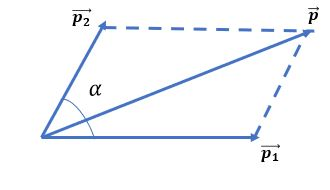
\includegraphics[scale=0.6]{../figs/VN10-PH-29-L-021-2-9.JPG}
			\end{center}
			\begin{itemize}
				\item Độ lớn động lượng của vật 1
				\begin{equation*}
					p_1=m_1v_1 =2\ \text{kg} \cdot \text{m/s}. 
				\end{equation*}
				\item Độ lớn động lượng của vật 2
				\begin{equation*}
					p_2=m_2v_2 =12\ \text{kg} \cdot \text{m/s}. 
				\end{equation*}
				\item Động lượng của hệ hai vật 
				\begin{equation*}
					\vec{p}=\vec{p_1}+\vec{p_2}.
				\end{equation*}
				Do vector động lượng của 2 vật tạo với nhau một góc $\alpha = 60^\circ$ nên độ lớn động lượng của hệ tính bởi 
				\begin{equation*}
					p= \sqrt{p_1^2+p_2^2 +2p_1p_2\cos \alpha}\approx 13\ \text{kg} \cdot \text{m/s}.
				\end{equation*}
			\end{itemize}
			\textbf{Đáp án: C.}}
	}
\end{dang}
\begin{dang}{Xác định độ biến thiên động lượng}
	\viduii{2}{Một quả bóng khối lượng $\SI{500}{g}$, chuyển động theo phương ngang với tốc độ $\SI{10}{m/s}$. Sau khi đập vuông góc vào một bức tường, quả bóng bật trở lại theo phương tới với tốc độ như cũ. Tính độ lớn của độ biến thiên động lượng của quả bóng.
	}
	{	\hide{	Chọn chiều dương là chiều chuyển động ban đầu của quả bóng. 
			
			Lúc đầu bóng có vận tốc $v_1=\SI{10}{\meter/\second}$ nên có động lượng lúc đầu của bóng 
			\begin{align*}
				p_1=mv_1=\SI{0.5}{\kilogram}\cdot\SI{10}{\meter/\second}=\SI{5}{\kilogram\cdot\meter/\second}.
			\end{align*} 
			Sau khi va chạm với tường, bóng chuyển động ngược chiều dương nên có vận tốc $v_2=\SI{-10}{\meter/\second}$ tương ứng với động lượng 
			\begin{align*}
				p_1=mv_2=\SI{0.5}{\kilogram}\cdot\left(\SI{-10}{\meter/\second}\right)=\SI{-5}{\kilogram\cdot\meter/\second}.
			\end{align*}
			Độ biến thiên động lượng của quả bóng:
			\begin{align*}
				\Delta p=p_2-p_1=\SI{-5}{\kilogram\cdot\meter/\second}-\SI{5}{\kilogram\cdot\meter/\second}=\SI{-10}{\kilogram\cdot\meter/\second}.
			\end{align*}
			Vậy độ lớn của độ biến thiên động lượng của bóng là \SI{10}{\kilogram \cdot\meter/\second}.}
	}
	\viduii{2}{Một vật khối lượng 1 kg rơi tự do với gia tốc $\text{9,8}\ \text{m/s}^2$ từ trên cao xuống trong khoảng thời gian 0,5 s. Chọn chiều dương hướng thẳng đứng từ trên xuống. Khi đó, độ lớn xung lượng của lực tác dụng lên vật trong khoảng thời gian nói trên bằng
		\begin{mcq}(2)
			\item $\SI{5}{\kilogram\cdot\meter/\second}$.
			\item $\SI{4.9}{\kilogram\cdot\meter/\second}$.
			\item $\SI{10}{\kilogram\cdot\meter/\second}$.
			\item $\SI{0.5}{\kilogram\cdot\meter/\second}$.
		\end{mcq}
	}
	{\hide{	Độ lớn xung lượng của lực
			\begin{equation*}
				F \Delta t = mg \Delta t =\SI{4.9}{\kilogram\cdot\meter/\second}.
			\end{equation*}
			\textbf{Đáp án: B.}}
	}
\end{dang}

\begin{dang}{Xác định độ biến thiên vận tốc, lực, khoảng thời gian mà lực tác dụng}
	\viduii{2}{Một chiếc xe khối lượng 100 kg đang đỗ trên mặt sàn phẳng nhẵn nằm ngang. Tác dụng lên xe một lực đẩy 800 N theo phương ngang để xe chuyển động về phía trước trong khoảng thời gian 2 s thì độ biến thiên vận tốc của xe trong khoảng thời gian này có độ lớn bằng
		\begin{mcq}(4)
			\item 1,6 m/s.
			\item 0,16 m/s.
			\item 16 m/s.
			\item 160 m/s.
		\end{mcq}
	}
	{\hide{	Chọn chiều dương là chiều chuyển động của xe lúc đầu.\\
			Dạng khác của định luật II Newton:
			\begin{equation*}
				\vec{F}\Delta t= \Delta \vec{p} =m \Delta \vec{v} \quad\Rightarrow\quad \Delta \vec{v} = \dfrac{\vec{F} \Delta t}{m}.
			\end{equation*}
			Suy ra độ lớn của độ biến thiên vận tốc 
			\begin{equation*}
				\Delta  v=\dfrac{F\Delta t}{m}=\dfrac{\SI{800}{\newton}\cdot\SI{2}{\second}}{\SI{100}{\kilogram}}= 16\ \text{m/s}.
			\end{equation*}
			
			\textbf{Đáp án: C.}}
	}
	\viduii{3}{
		Một quả bóng $\SI{2.5}{\kilogram}$ đập vào tường với tốc độ $\SI{8.5}{\meter/\second}$ và bị bật ngược trở lại với tốc độ $\SI{7.5}{m/s}$. Biết thời gian va chạm là $\SI{0.25}{\second}$. Tìm lực mà tường tác dụng lên quả bóng.
	}
	{\hide{Chọn chiều dương là chiều chuyển động lúc đầu của quả bóng. 
			
			Độ biến thiên động lượng của quả bóng:
			$$\Delta p =p_2-p_1=mv_2-mv_1=\SI{2.5}{\kilogram}\cdot(\SI{-7.5}{\meter/\second})-\SI{2.5}{\kilogram}\cdot\SI{8.5}{\meter/\second}= \SI{-40}{kg.m/s}.$$
			
			Lực mà tường tác dụng lên quả bóng: $$F=\dfrac{\Delta p}{\Delta t} =\dfrac{\SI{-40}{\kilogram\meter/\second}}{\SI{0.25}{\second}}= \SI{-160}{N}.$$
			Vậy: lực tác dụng có độ lớn $\SI{160}{\newton}$ lên quả bóng và ngược chiều chuyển động ban đầu của bóng.}
	}
\end{dang}